%Copyright (C) 2016 by Krishneel@JSK Lab, The University of Tokyo

\documentclass{standalone}
\begin{document}

\subsection{Platforms}

For task 3, we developed two types of UAV. We first used customized
DJI M100 as our standard platform (Fig. \ref{task3platform-m100}), which has
been introduced in task 1. The UAV is equipped with Nvidia Jetson TX1
and TK1 based embedded computers to run control and vision
algorithms. 
We re-designed the magnetic gripper with improved strength and
reinforcements for picking up a variety of objects. In addition, the UAV is
more stable with the newer design as drag is reduced.
For the second type of UAV, we improved the transformable aerial robot called
{\bf Hydrus} (Fig. \ref{task3platform-hydrus}) which was described in the first
report. The propellers of {\bf Hydrus} are 14[inches] which is longer
than the prototype. As a result the flight performance is
improved. Temporarily we used the standard platform via remote operation to
perform real world tests. Also, we are trying to setup the network
configurations according to the requirements of the competition. 

%% Also we accelerate
%% our vision algorithm in gazebo simulation
%% as we showed in the first report. For now we are trying to develop a
%% semi-autonomous approach for task 3 considering the difficulties we
%% meet in manually operation.


 \begin{figure}%[hb]
    \begin{center}
    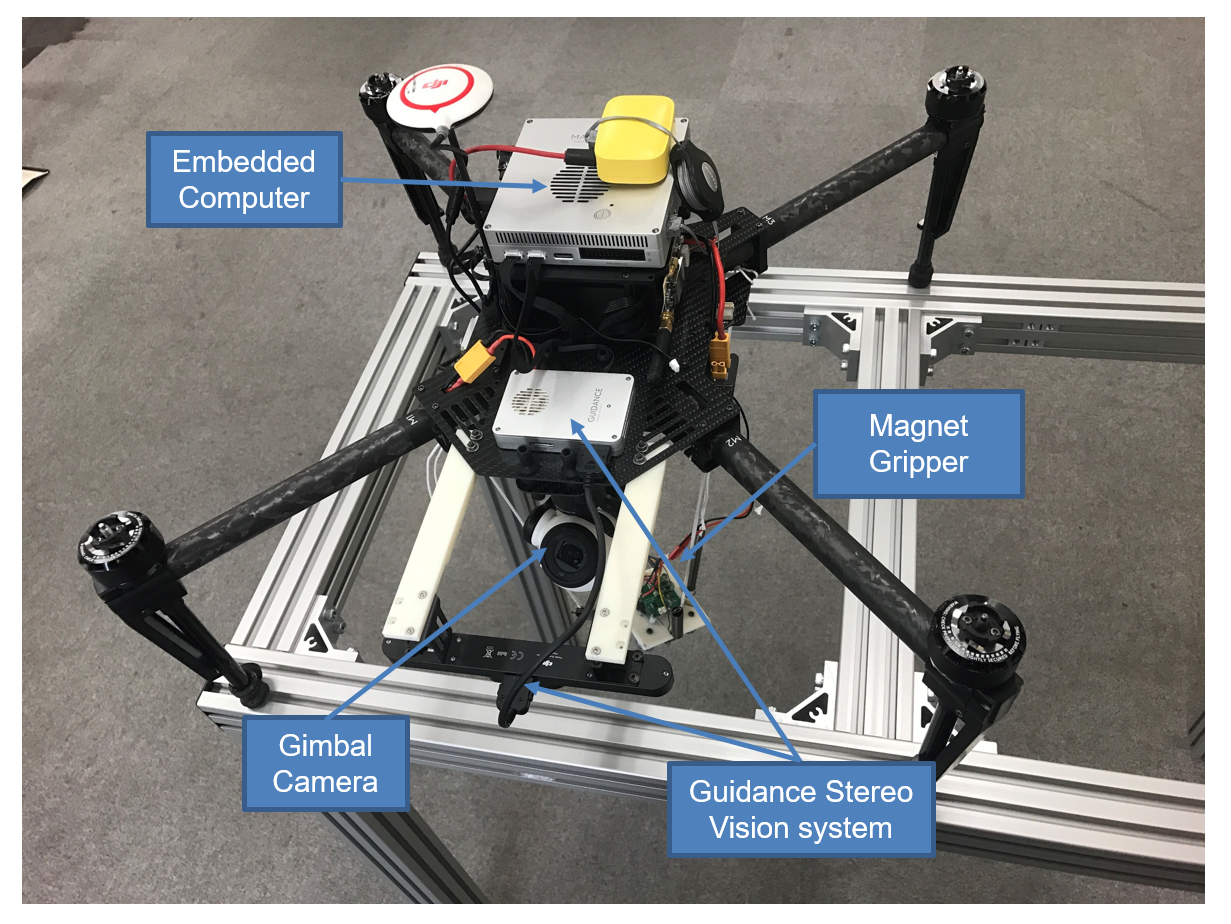
\includegraphics[keepaspectratio=true, width=1\linewidth, height=0.3\textheight]
    {sections//task3//images//task3platform.png}
      \end{center}
    \caption{Task 3 Platform: DJI M100}
    \label{task3platform-m100}
    \end{figure}
 \begin{figure}%[hb]
    \begin{center}
      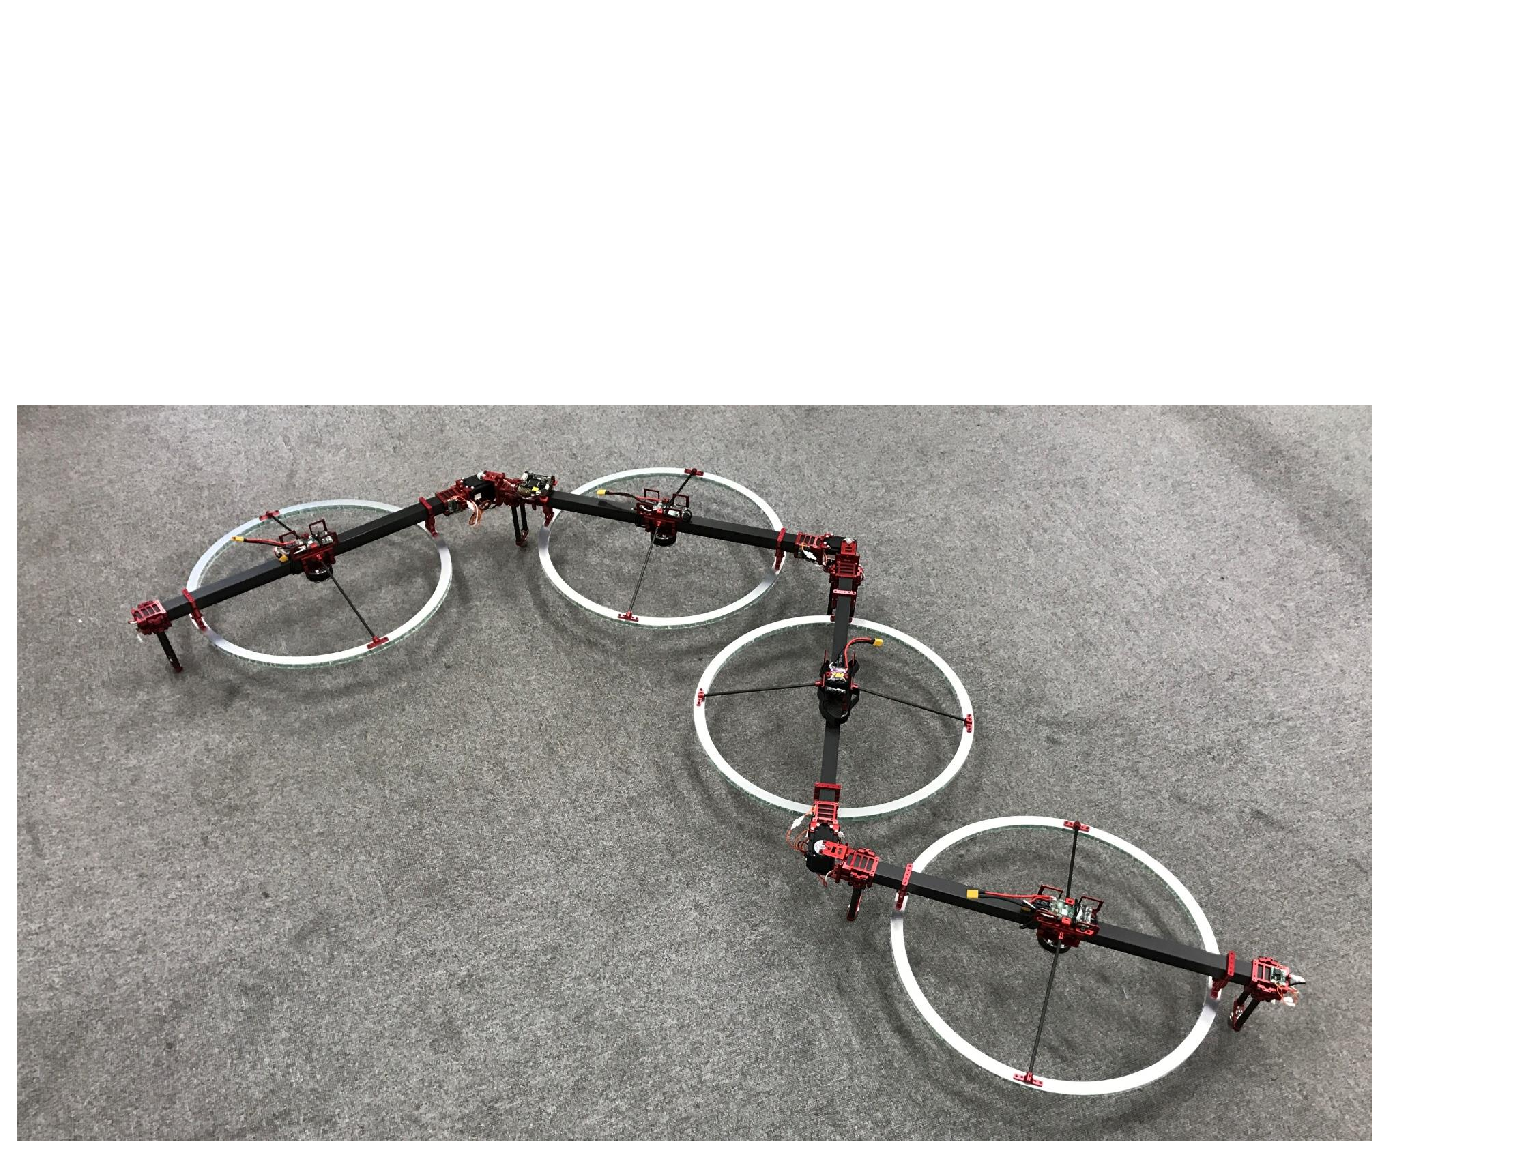
\includegraphics[clip, bb= 0 0 650 350, width=\columnwidth]{sections/task3/images/task3platform-hydrus.eps}
      \end{center}
    \caption{Task 3 Platform: Hydrus}
    \label{task3platform-hydrus}
    \end{figure}
    
    
\subsection{Electromagnet Gripper for Quadcopter}

We chose to use an electromagnet gripper based on its ease of control, and also because the circuits
can be readily designed and made by ourselves. Permanent magnets are stronger but it also
requires an extra mechanism to push on the object for releasing, which will
make the attachment more complex, and may also require an additional motor. We
also contemplated on the use of an air vacuum but the size of a vacuum is too
big for our drone.

 \begin{figure}[hb]
    \begin{center}
    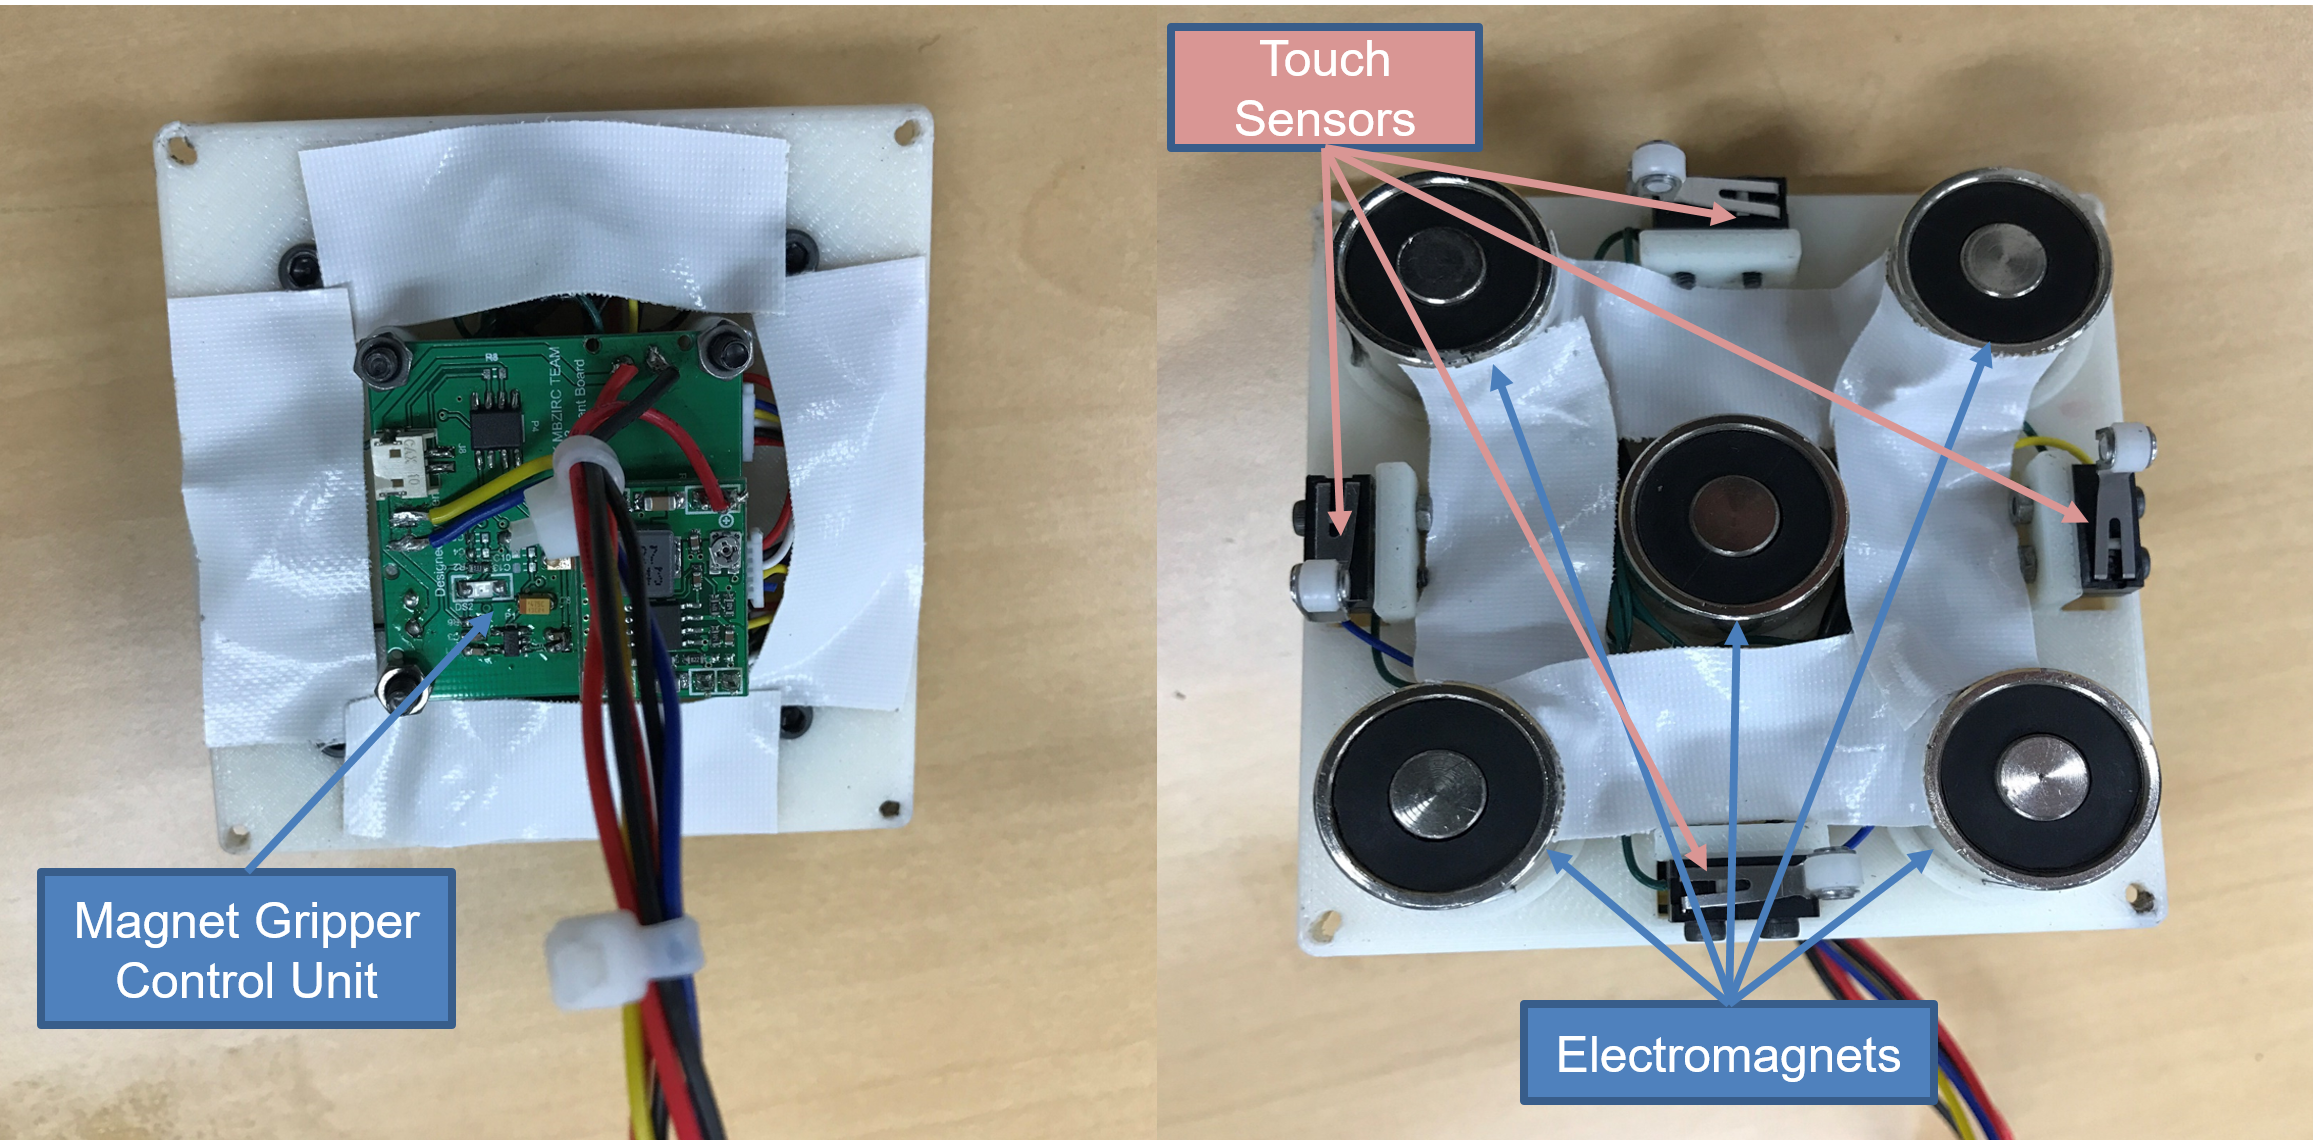
\includegraphics[keepaspectratio=true, width=1\linewidth, height=0.3\textheight]
    {sections//task3//images//task3gripper.png}
      \end{center}
    \caption{Task 3 Gripper($8cm \times 8cm, 240g$)}
    \label{task3platform}
    \end{figure}

We equipped 5 small electromagnets on a gripper of size $8cm \times
8cm$. Each electromagnet is capable of producing more than $20 N$
of attractive force given a good object thickness. The gripper shown in
Fig.\ref{task3platform} consisting of $5$
electromagnets can pick up an object made of iron weighing near $1kg$ with a thickness of more than $0.3mm$.
The gripper is also equipped with four touch sensors to detect
object--gripper contact state. In addition,
these touch sensors are used to determine the position of the gripper
with respect to the object. 
%% For instance if $2$ or $3$ touch sensors
%% are triggered and then we know the offset of the gripper and the
%% object. 

%% However, according to our experiment,
%% since each object is less than $500 g$, the thickness will be less
%% than $1.6 mm$ if the object is a square of $20cm \times 20cm$ and made
%% of pure iron(consider the density of iron to be $7.86 g/cm$). 
%% In
%% addition, if the surface of the object is too large, the propeller
%% effect will happen and therefore request the electromagnets to be more
%% powerful. Temporary our gripper with $5$ electromagnets can pick the
%% object of almost $1kg$ of the thickness of the iron is more than
%% $0.3mm$. 


 \begin{figure*}%[hb]
    \begin{center}
    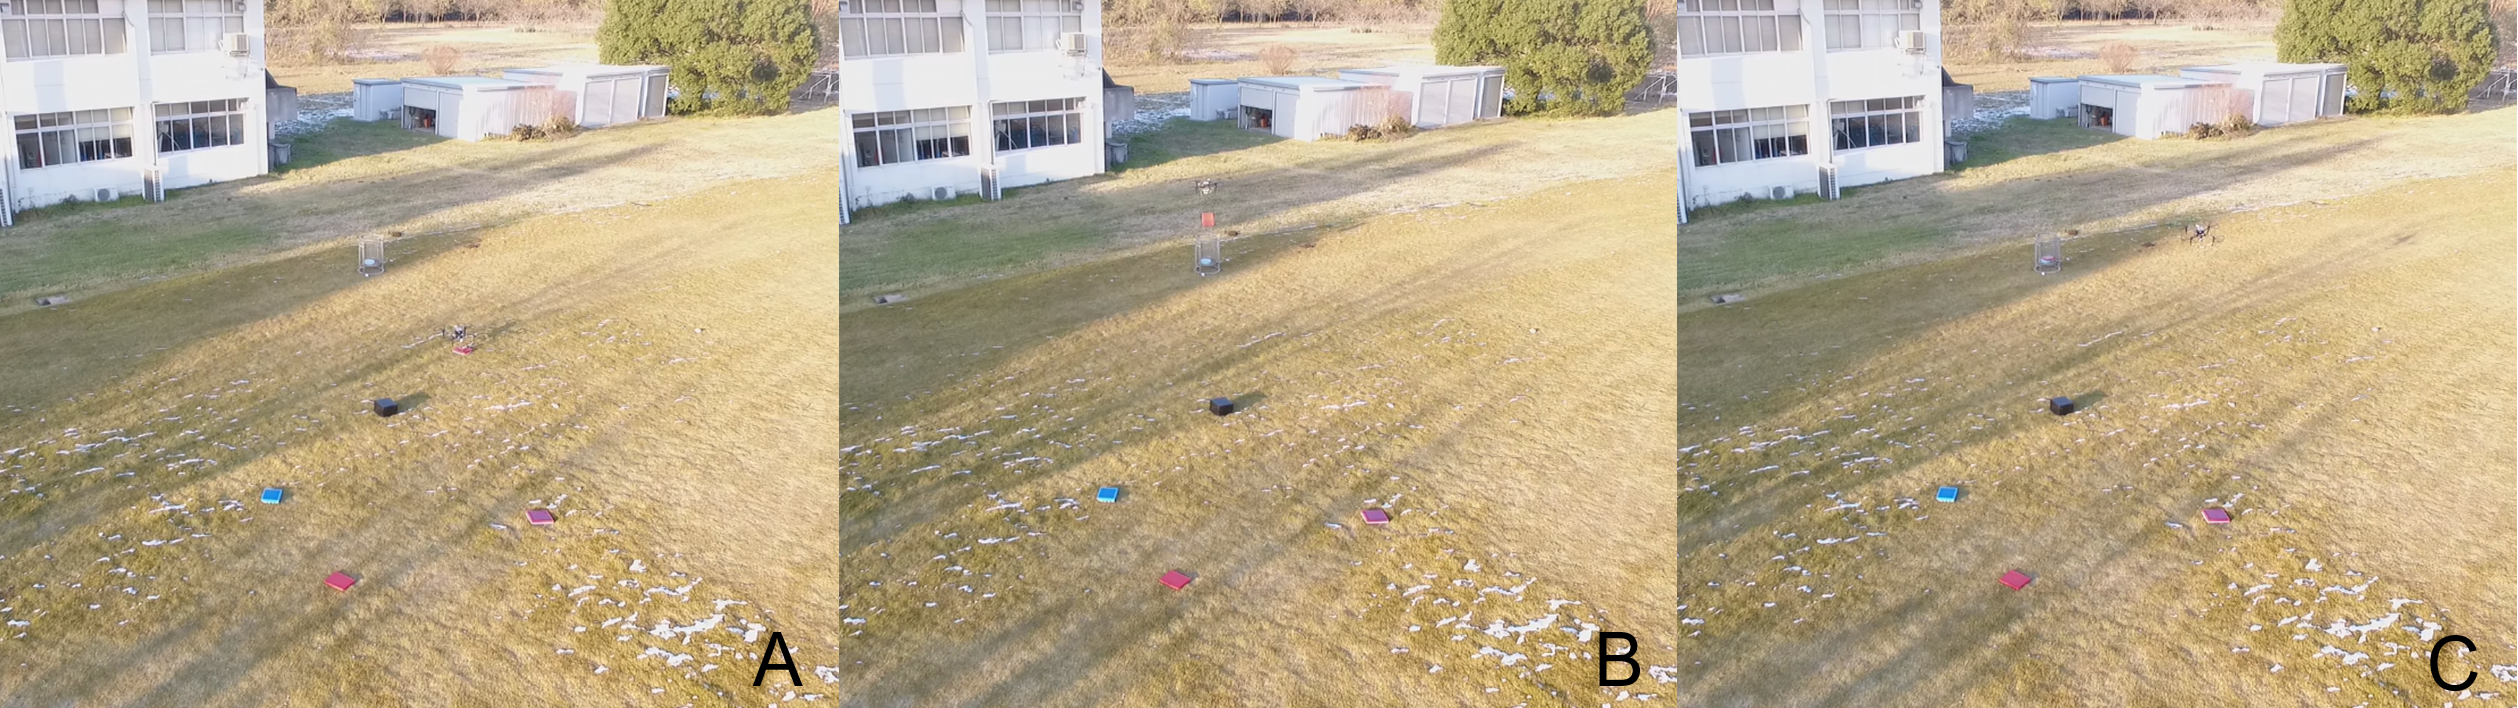
\includegraphics[keepaspectratio=true, width=1\linewidth, height=0.3\textheight]
    {sections//task3//images//teleop.png}
      \end{center}
    \caption{Pick, Place and Search in Teleoperation(A: Pick an object, B: Place the object back to a tray box, C: Search and approach to an object)}
    \label{task3tele}
    \end{figure*}

    
The design of the electromagnet circuits driver is simple since it can
be simply regarded as a series connection of a inductor and a small
resistor. Darlington Transistor is suitable to drive an
electromagnet as the current requirement is only $200 ma$. Because of
the inductor effect, a protection diode is necessary in the
circuits to prevent backflow. We designed the circuits board with a
$32$ bits micro controller, a Darlington driver IC and both serial, CAN communication
interface in the gripper board. An on-board driver written as a ROS node
collects the status of the magnets and the touch sensors in the
gripper and reports these information to the embedded computers.

%% on board driver written on ROS
%% the status of the magnets and the touch sensors in the gripper can be
%% collected and reported 
%% it can directly report the status of the magnets and touch sensors in
%% the gripper and also receive the orders from the embedded computers. 


\subsection{Teleoperation for Task 3}

We performed experiments using the aforementioned hardware equipped
onto the UAVs. The UAVs were controlled through tele--operation. The
software which were implemented on the simulator needed
fine-tuning to operate in the real world. Approaching the object for
grasping is relatively difficult due to rapid visual changes. A more
crucial problem when approaching the object is the ground effect which 
results in unexpected behaviour and the UAV becomes unstable very
quickly. We addressed this problem by suspending the magnet gripper with
a spring so that the UAV can pick the object without getting too close
to the ground. However this introduces another problem, i.e., 
the gripper shaking whenever the UAV changes its velocity. We are
currently working towards alleviating the problem.



%% When we control the UAV manually to
%% pick the object, we figure out it is not a easy job for real UAV
%% platform compared to the simulation since it is very difficult to
%% control the UAV accurately to approach the object, in addition, the
%% ground effect will unstable the UAV when the UAV is getting close to
%% the ground. We address this problem by hanging the magnet gripper with
%% a spring so that the UAV can pick the object without getting too close
%% to the ground. However this may introduce another problem that the
%% gripper will be shaking whenever the UAV change the velocity, we are
%% also addressing this problem now and try to get a stronger hanging
%% method to make the gripper relatively stable.

%% At this moment, we only perform the real platform experiment through
%% teleoperation by human beings. When we control the UAV manually to
%% pick the object, we figure out it is not a easy job for real UAV
%% platform compared to the simulation since it is very difficult to
%% control the UAV accurately to approach the object, in addition, the
%% ground effect will unstable the UAV when the UAV is getting close to
%% the ground. We address this problem by hanging the magnet gripper with
%% a spring so that the UAV can pick the object without getting too close
%% to the ground. However this may introduce another problem that the
%% gripper will be shaking whenever the UAV change the velocity, we are
%% also addressing this problem now and try to get a stronger hanging
%% method to make the gripper relatively stable.

\subsection{Results}

We performed experiments using one UAV, the standard platform. 
%We tested on one UAV and it seems 
On average we can pick $5$ static objects within $8$ minutes. The time
can be improved if we adopt a 
semi-autonomous teleoperation method, in which we store the global position of
the box to drop the objects, so that after picking the object, the UAV can
directly move to the global position of the drop box by itself.


\subsection{Future Work}
In the next step of task 3 we are going to improve our vision
detection method. While the performance of these algorithms yield good
results in simulation, they still need improvements when applying to
the real world. With improvements in the vision algorithms and reduction
in gripper vibration and oscillation, we will make the task3 fully autonomous. In addition, we will design a multi UAVs cooperation strategy for
task 3, both for teleoperation and full autonomy.


\end{document}
